%%%%%%%%%% %%%%%%%%%% %%%%%%%%%% %%%%%%%%%% 
\section{Implementation and Evaluation}
\label{sec:05Implementation}

% Text matter begin
%%%%%%%%%% %%%%%%%%%% %%%%%%%%%% %%%%%%%%%% 
\subsection{Implementation Details}
\label{subsec:implementation}
We implement \design{} in Python (about 6,000 lines of code), mainly using PyTorch for ML operations and FAISS for high-speed vector similarity search. A key optimization is to place the model weights and intermediate tensors in a shared memory region, so that multiple processes in the same pipeline stage can load them without duplicating. This reduces overall memory usage by $\sim$70\% compared to loading models into each process privately, and with minimal synchronization overhead. To manage parallel execution across pipeline stages, we avoid Python’s \texttt{ThreadPoolExecutor} and use a \texttt{ProcessPoolExecutor} configuration along with explicit CPU-core pinning. This approach circumvents the Global Interpreter Lock, ensures genuine parallelism on each CPU core, and reduces cache misses by lowering context-switch overhead. In the encoding stage, we store the embeddings in contiguous arrays via \texttt{np.ascontiguousarray()}, which helps to exploit SIMD-based vector instructions more effectively.

\noindent\textbf{Deployment System:} \new{Following \Cref{sec:BG:Scope}, our evaluations span two local/personal-computing platforms and one embedded device:} (1) An Intel i9-14900K platform~\cite{intel_cpu} with 32 virtual cores (8 P-cores and 16 E-cores) and 128\,GB of main memory, paired with an RTX\,4090 GPU~\cite{nvidia_rtx_gpu} with 24\,GB of VRAM; (2) An Intel i9-14900F with the same CPU-core configuration but connected to an RTX\,4080 GPU with 16\,GB of VRAM; and (3) An Nvidia Jetson~AGX Orin development kit with 64\,GB of unified memory \cite{nvidia_jetson_orin}, where we cap its power budget at the lowest provisioned state of 15W.
\new{All three are personal-computing edge nodes in the sense of \Cref{sec:BG:Scope}: each runs RAG locally for a single user, without cloud intervention, under limited power and compute budgets. On the Jetson the budget is explicit: the 15W cap leaves 4 of its 12 CPU cores available.}
%for experiments.

\noindent\textbf{Dataset and Traces:} We used the Wikipedia corpus dump \cite{wikipedia_corpus_dump} as our knowledge source and relied on the FAISS library \cite{faiss} to build a \emph{flat index} that uses an L2-distance measure for \topk similarity searches. Query prompts are drawn from Google’s Natural Question Dataset \cite{natural_questions}. Because there is no publicly available trace for RAG workloads on personal devices, we downscaled bursty traces from Azure to better approximate smaller, consumer-grade computing capabilities. For the similarity search process, we use flat indices to obtain the \topk most similar elements. The text embedding model used in all experiments is \texttt{e5-base-v2} \cite{e5_base_v2}. For the generation stage, we used Llama-3.1-8B-Instruct \cite{llama_3_1_8b_instruct} and OPT\,2.7B \cite{opt} on the RTX\,4090 and RTX\,4080, respectively, and a smaller Llama-3.2-1B \cite{llama3_2_1b} in Jetson Orin, where we impose a 15W power limit.

\noindent\textbf{Metrics:} We report two key performance metrics for the end-to-end pipeline. The first is "latency", which is the total completion time for a batch of queries. The second is "throughput" (qps), defined as the number of queries processed per second. In the results, we compare our proposed \design{} against three baseline approaches: (1) FlashRAG~\cite{jin2024flashrag}--presents a modular RAG framework where both encoding and generation are placed on the GPU; (2) PipeRAG~\cite{jiang2024piperag}--a server-oriented pipeline design; and (3) EdgeRAG~\cite{EdgeRAG}--mitigates memory usage by caching only coarse indices and generating finer embeddings on demand using the GPU.
%focuses on on-demand GPU encoding for edge computing. 
To ensure that the proposed orchestration fits in the tight power and energy constraints of \new{the personal-computing edge platforms}, we report the peak and average power (in W) and the total energy (in J) consumed per inference query.

%\red{To assess the real-world feasibility of our proposed solution in terms of energy consumption on edge platforms, we conduct comprehensive power profiling of both CPU and GPU components, with results presented in Section~\S\ref{sec:overallLatencyPower}. For CPU power measurement, we employ \texttt{turbostat} utility~\cite{turbostat}, which provides hardware-based power consumption data by accessing model-specific registers (MSRs) and Running Average Power Limit (RAPL) counters. This approach delivers package-level and core-level power measurements with sampling at 10Hz frequency. GPU power consumption is measured using NVIDIA's System Management Interface (\texttt{nvidia-smi}), which queries onboard power sensors to obtain instantaneous power draw measurements at 20Hz sampling frequency. Both measurement techniques utilize dedicated hardware counters, ensuring high accuracy ($\pm1-5\%$ for CPU, $\pm2-3\%$ for GPU) for our power consumption analysis. For the Jetson platform, we cap the power to 15W only which is the lowest power setting offered on the particular platform representative of the handheld mobile devices used everyday.}
%All these prior studies  are evaluated against \design{} to highlight performance differences using the metrics chosen.

% \subsection{Implementation Details}
% We implemented \design{}, leveraging PyTorch's computational infrastructure. Our codebase consists of approximately 6,000 lines of code, utilizing PyTorch for ML operations and FAISS for accelerated vector similarity search. We utilize PyTorch's shared memory function to ensure model weights and intermediate tensors are shared across multiple worker processes of the same stage, eliminating redundant memory allocation. 
% Our benchmarks revealed memory savings of up to 70\% compared to individual process loading with negligible synchronization overhead. For concurrent execution of pipeline stages, we employ Python's \texttt{ProcessPoolExecutor} rather than the more commonly used \texttt{ThreadPoolExecutor}. This design choice enables parallel processing across CPU cores, while avoiding the limitations of Python's Global Interpreter Lock (GIL). We complement this with explicit CPU core pinning, which reduces context switching overheads and improves cache locality. In the encoder, we implement a contiguous memory layout for embeddings using \texttt{np.ascontiguousarray()}, which enables more efficient SIMD vectorization operations.

% \noindent\textbf{Hardware Setup}: We perform experiments on 
%  three different hardware setups representative of the different consumer and edge grade devices: (i) Intel i9-14900K having 32 virtual cores (8 P-cores and 16 E-cores constituting the 24 physical cores) with 128 GB main memory, equipped with RTX 4090 GPU with 24 GB memory; (ii) Intel i9-14900F having aforementioned CPU core configuration and connected to an RTX 4080 GPU with 16 GB memory; and (iii) Nvidia Jetson AGX Orin developer kit with 64 GB main memory~\cite{nvidia_jetson_orin}. These devices are representative of the personal computing/edge devices available to the users today. 

% \noindent\textbf{Datasets and Models}: We use Wiki corpus dump~\cite{wikipedia_corpus_dump} for knowledge retrieval database and it is indexed using FAISS library~\cite{faiss} to create a flat indexing scheme where "L2 distance" is used as a similarity metric for top k item selection with respect to the input prompt. The input prompts used for query are from Google's Natural Question Dataset~\cite{natural_questions}. Since there is no publicly available trace representative of RAG use-pattern on personal computing devices, we use bursty traces from Azure scaled down to fit smaller computational footprint matching the consumer-grade device capabilities. The text-to-embedding generation model used to generate the embeddings for the database and the incoming queries is e5-base-v2\cite{e5_base_v2}. The models used for inference are Llama-3.1-8B-Instruct\cite{llama_3_1_8b_instruct} and OPT 2.7B\cite{opt} on the RTX 4090 and RTX 4080 GPUs, respectively. We choose a smaller model Llama-3.2 1B\cite{llama3_2_1b} model to run on Jetson AGX Orin development board. For Jetson Orin evaluations, we cap the power budget at 15W.

% \noindent\textbf{Metrics}: 
% %Since the target application is mostly user facing on a resource constrained personal computational platform, 
% We use (i) latency and (ii) throughput as the primary metrics in our evaluations. Latency is defined as the time it takes for a batch to finish the end-to-end RAG application, and throughput is defines as Queries served per second (qps).
% %For Jetson Orin evaluations, we cap the power budget at 15W.

% \noindent\textbf{Design schemes}: The baselines chosen to compare the proposed design against are (i) FlashRAG\cite{jin2024flashrag} which presents an end-to-end RAG pipeline and evaluation framework where the encoding and generation stages take place on GPU, (ii)  PipeRAG\cite{jiang2024piperag} that introduces pipelining at server-scale computing, and EdgeRAG \cite{}. We compare all the baselines with "\design{}"
% %Note that none of these prior approaches  addresses the underlying resource aware task mapping issue,  which becomes even more critical in personal computational devices like laptops, tablets, and smartphones where computational resources are scarce.


% \textbf{Latency Results on Consumer Grade Systems}
% \label{subsec:eval4090}
% We next present our end-to-end latency measurements and compare against three baselines on three distinct hardware platforms: two consumer-grade desktop systems (one with an \mbox{RTX\,4090} and another with an \mbox{RTX\,4080}) and an embedded-class Jetson~AGX~Orin device. We study both raw latency (i.e., time-to-finish for a single batch) and the speedup ratio of our approach over the baselines. In each set of experiments, we use the same model pipelines as the baselines---EdgeRAG, FLashRAG, and FLashRAG---and, where applicable, reuse or replicate their model configurations. Our goal is to highlight how careful CPU--GPU partitioning and fine-grained pipeline design can improve end-to-end performance across a variety of real-world problem scales.

% \subsection{Results on \mbox{RTX\,4090} and \mbox{RTX\,4080} Desktop:}
% \label{subsec:eval4090}
% \noindent\textbf{Overall Latency and Speedups on RTX 4090.}
% \Cref{Fig:OurLatencyE2E4090} shows the raw latency of our design on the \mbox{RTX\,4090} as we vary batch size from~2 to~16 and database size from~1\,million to~8\,million. We see that the latency naturally grows with both batch size and database scale: larger batches mean more encoding and generation work, while bigger databases make retrieval (an I/O-heavy task) more time-consuming. Even for the largest configuration (\texttt{BS=16}, \texttt{DB=8\,M}), we remain feasible on an \mbox{RTX\,4090}, finishing the batch in about 25\,s.

% In \Cref{Fig:Lat-vs-EdgeRAG}--{\ref{Fig:Lat-vs-PipeRAG}, we d}epict our speedup over EdgeRAG, FLashRAG, and FLashRAG, respectively. We see that our design delivers marked gains across every configuration. For instance, compared to EdgeRAG [\Cref{Fig:Lat-All-4090}(b)], we observe up to a $\approx12\times$ faster execution at \texttt{BS=8}, \texttt{DB=8\,M}. As the batch size increases from~2 to~8 (particularly at mid-scale database sizes, 2--4\,M), the advantage becomes more pronounced, due to EdgeRAG's frequent GPU model loading and CPU--GPU transfers. Our pipeline, by contrast, executes encoding on the CPU in a more memory-friendly manner and avoids redundant data movement. At \texttt{BS=16}, \texttt{DB=8\,M}, our speedup dips to about $6.15\times$, reflecting partial I/O saturation in retrieval, yet it still significantly outperforms the baseline.

% Against FLashRAG [\Cref{Fig:Lat-All-4090}(c)], we likewise see speedups from about $2\times$--$3\times$ at moderate batch sizes, and up to $3.15\times$ at the largest sizes. A notable anomaly is that FLashRAG tends to run out of memory around \texttt{BS=16} and moderately large databases, whereas our pipeline completes successfully, underscoring the advantage of assigning retrieval and encoding to the CPU. Similarly, FLashRAG [\Cref{Fig:Lat-All-4090}(c)] faces repeated GPU--CPU handoffs, resulting in pipeline stalls. While it attempts some pipeline concurrency, it still offloads too many stages to the GPU. For larger batches, FLashRAG also experiences memory exhaustion, whereas our system remains robust up to \texttt{BS=16} and \texttt{DB=8\,M}.

% \noindent\textbf{ Insights.}
% Two major lessons emerge from \Cref{Fig:Lat-All-4090}. 
% First, partitioning CPU and GPU tasks carefully is crucial: forcing both encoder and generative model onto the GPU triggers heavy data transfers and repeated model loads. 
% Second, moderate batch sizes (\texttt{BS=4--8}) typically provide the most efficient balance of I/O and compute; pushing too high eventually saturates I/O or memory, but staying too low underutilizes resources. 
% Overall, from a \emph{designer’s perspective}, sweet-spot batching and CPU--GPU division together yield 6$\times$--12$\times$ latency gains over existing designs without risking out-of-memory failures.

% %\subsection{Results on an \mbox{RTX\,4080} Desktop}
% %\label{subsec:eval4080}
% \noindent\textbf{Results on an \mbox{RTX\,4080} Desktop:}
% \Cref{Fig:4080Latency_Ours} reports the raw latency of our design on the \mbox{RTX\,4080} platform, sweeping batch size (2--16) and database size (1--8\,M). The results mirror those on the \mbox{RTX\,4090}: our end-to-end latency scales acceptably with increasing batch and database sizes, peaking at around 11.58\,s for \texttt{BS=16} at 8\,M entries. In \Cref{Fig:4080Speedup_Merged}, we show our speedup over EdgeRAG, FlashRAG, and FLashRAG at a moderate database size of 4\,M. For \texttt{BS=2}--\texttt{BS=8}, we outperform each baseline significantly, showing up to $8.97\times$, $3.08\times$, and $5.80\times$ improvements, respectively. 
% All baselines are unable to complete \texttt{BS=16} for 4\,M entries due to memory exhaustion on this 16\,GB GPU. In contrast, by relegating only the generation stage to the GPU, our pipeline avoids large GPU memory footprints and finishes \texttt{BS=16} successfully. 
% From these observations, we infer that a naive GPU-offloading approach easily becomes infeasible for moderately large batch sizes, affirming that CPU-based encoding and retrieval are more sustainable for midrange GPUs.

\subsection{\texorpdfstring{\new{Stage-Level Latency Breakdown}}{Stage-Level Latency Breakdown}}
\label{sec:breakdown}
\begin{table}[t]
\centering
\caption{\new{Stage-level latency in seconds on the RTX\,4090 at \texttt{DB=4\,M} and \texttt{BS=8}, with caching disabled. Generation is excluded because its settings are common to all four systems. A spanned cell marks stages a system measures together: \design{} and \edgeRAG{} fuse retrieval and augmentation (\Cref{subsec:pipeline_design}), while \flashRAG{} fuses encoding and retrieval. An empty cell marks a cost the system does not report separately.}}
\label{tab:latency_breakdown}
{\small
\setlength{\tabcolsep}{3pt}
\begin{tabular}{lccccc}
\toprule
\textbf{System} & \textbf{Enc.} & \textbf{Retr.} & \textbf{Aug.} & \makecell{\textbf{Model}\\\textbf{loads}} & \makecell{\textbf{Sched.}\\\textbf{/ sync}} \\
\midrule
\design{}   & 0.20 & \multicolumn{2}{c}{1.60}  &                              & 0.20 \\
\edgeRAG{}  & 0.28 & \multicolumn{2}{c}{25.19} &                              &      \\
\flashRAG{} & \multicolumn{2}{c}{7.26} & 0.10  & \makecell{0.73 enc.\\2.20 LLM} &      \\
\pipeRAG{}  & 6.20 & 5.20 & 0.10            &                              & $\leq 2$ \\
\bottomrule
\end{tabular}%
}
\end{table}

\begin{newtext}
\Cref{tab:latency_breakdown} decomposes the per-stage cost of \design{} and the three baselines at a common operating point. Generation is excluded because its settings are the same for all four systems, so it is not a source of difference between them. Caching was disabled for these measurements and for the primary results reported in this section. \edgeRAG{} spends 25.19\,s in fused retrieval and augmentation, which is the cost of generating embeddings on demand. \flashRAG{} pays 0.73\,s to load the encoder and a further 2.20\,s to load the LLM, which are model reloads. \pipeRAG{} measures the three CPU stages separately but pays up to 2\,s in synchronization, serialization, and timeout, which is contention between stages. \design{} reports 0.20\,s for encoding, 1.60\,s for fused retrieval and augmentation, and 0.20\,s of scheduler cost.
\end{newtext}

\subsection{Results on \mbox{RTX\,4090} and \mbox{RTX\,4080} Desktop}
\label{subsec:eval4090}
\noindent\textbf{Overall Latency and Speedups on RTX\,4090:}
\Cref{Fig:OurLatencyE2E4090} plots the end-to-end latency of our design on an \mbox{RTX\,4090} across batch sizes of 2--16 and database sizes of 1--8\,million. As batch size or database size grows, the latency increases because larger batches demand more encoding and generation while bigger databases incur heavier I/O in retrieval. Even in the largest case (\texttt{BS=16}, \texttt{DB=8\,M}), our approach remains feasible, completing in  \emph{$\approx25\,s$}. In \Cref{Fig:Lat-vs-EdgeRAG}--\ref{Fig:Lat-vs-PipeRAG}, we show speedups over EdgeRAG, FlashRAG, and PipeRAG, respectively, and observe consistent gains. Compared to EdgeRAG [\Cref{Fig:Lat-All-4090}(b)], we see up to a $\approx12\times$ speedup at \texttt{BS=8}, \texttt{DB=8\,M}, primarily because our CPU-based encoding avoids redundant GPU transfers. In higher batches, the speedup drops slightly (e.g., to $6.15\times$ at \texttt{BS=16}, \texttt{DB=8\,M}) due to partial I/O saturation, but still substantially outperforms EdgeRAG. Against FlashRAG [\Cref{Fig:Lat-All-4090}(c)], we see gains of 2--3$\times$ and occasionally higher when larger batches make GPU memory usage critical; FlashRAG often runs out of memory for \texttt{BS=16}, whereas our CPU-side retrieval and encoding remain robust. These experiments highlight the importance of selecting which stages run on the GPU and which on the CPU. Pushing both encoder and LLM to the GPU triggers repeated data transfers and frequent model reloading, while moderate batch sizes (\texttt{BS=4--8}) help balance resource use. Overall, carefully partitioning CPU vs. GPU tasks and choosing middle-range batch sizes yields 6--12$\times$ faster processing without risking out-of-memory problems\new{; \Cref{sec:breakdown} decomposes these results by pipeline stage}.
%\noindent\textbf{ Insights.}
Two major lessons emerge from \Cref{Fig:Lat-All-4090}. 
First, partitioning CPU and GPU tasks carefully is crucial: forcing both encoder and generative model onto the GPU triggers heavy data transfers and repeated model loads. 
Second, moderate batch sizes (\texttt{BS=4--8}) typically provide the most efficient balance of I/O and compute; pushing too high eventually saturates I/O or memory, but staying too low underutilizes resources. 
Overall, from a \emph{designer’s perspective}, sweet-spot batching and CPU--GPU division together yield 6--12$\times$ latency gains over existing designs without risking out-of-memory failures.
%\textcolor{red}{We used flat-indexing for accuracy and benchmarked three popular alternatives—IVF-Flat, IVF-PQ, and HNSW—observing performance gains of 29.27\%, 28.15\%, and 32.18\%, respectively, wrt flat-indexing.} 

\noindent\textbf{Results on an \mbox{RTX\,4080} Desktop:}
\Cref{Fig:4080Latency_Ours} shows that, on \mbox{RTX\,4080}, our total latency follows a similar pattern, scaling to about 11.58\,s at \texttt{BS=16}, \texttt{DB=8\,M}. In \Cref{Fig:4080Speedup_Merged}, where we specifically compare speedups at \texttt{DB=4\,M}, batch sizes of 2--8 run successfully with \design{} but cause memory exhaustion in all baselines at \texttt{BS=16}. That reflects how naive GPU offloading can overwhelm the 16\,GB GPU memory if encoding and retrieval also reside there. 
In contrast, dedicating only generation to the GPU keeps our pipeline stable for larger batches. These results confirm that CPU-driven encoding and retrieval strategies are more sustainable for mid-range GPUs while still providing significant performance gains and avoiding failures on bigger inputs. 

% \subsection{Results on Jetson~AGX~Orin}
% \label{subsec:evalJetson} %old
% Finally, \Cref{fig:JetsonThemVsUs} compares our pipeline with EdgeRAG on a Jetson~AGX~Orin. Here we are limited to 4 CPU~cores at a 15\,W power cap, and we consider a smaller 1M database. Even under these constraints, our approach delivers consistent speedups, peaking at around $1.35\times$ for \texttt{BS=8}. At \texttt{BS=16}, resource saturation in both CPU and memory causes the speedup to taper off to $\approx1.25\times$. The absolute latency on Jetson is higher by nature (tens of seconds, rather than single-digit), but these results highlight two things: 
% (1)~our pipeline’s minimal CPU--GPU transfers remain advantageous even on low-power SoCs, and 
% (2)~models and indexing must be chosen carefully for memory-constrained settings. 

% %\noindent\textbf{Discussion.}
% The results on Jetson Orin further stress the importance of pipeline design for smaller devices. A naive GPU-based encoder would force repeated loading or large data transfers, quickly overwhelming limited DRAM. By mapping the encoder and retrieval to CPU workers and reusing memory-mapped indices, we mitigate these overheads. Although the speedups versus EdgeRAG are less dramatic than on a 4090/4080 (since the overall system is smaller), we still observe about $25\%$--$35\%$ latency reductions. These results suggest that \emph{even modest system-level refinements can pay off} in embedded-class deployments.

% %%%%%%%%%%%%%%%%%%%%%%%%%%%%%%%%%%%%%%%%%%%%%%%%%%%%%%
% \begin{figure}
% \centering
% 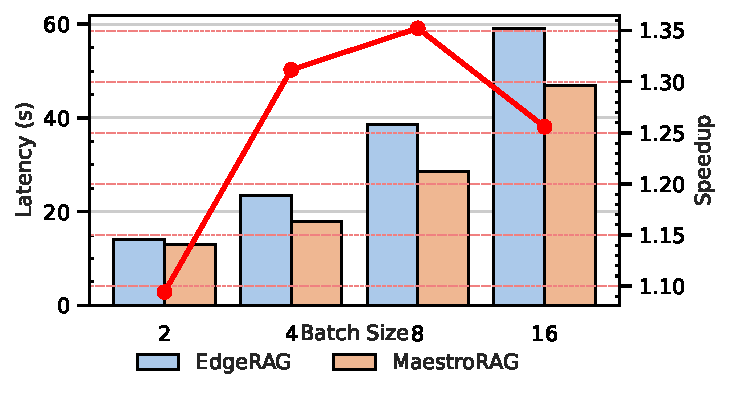
\includegraphics[width=0.9\linewidth]{Figs/JetsonThemVsUs.pdf}
% \caption{Latency comparison of EdgeRAG and \design{} on on Jetson AGX Orin with 15W power budget.
% %. We run 4-cores at a 15\,W power limit, with a 1\,M database, and \texttt{top-k}=5. We show both latencies (in seconds) and the resulting speedup as batch size increases. A maximum speedup of about 1.35$\times$ is observed at a batch size of 8,while performance gains at larger batch sizes taper due to resource saturation.
% }
% \label{fig:JetsonThemVsUs} 
% \end{figure}
% %%%%%%%%%%%%%%%%%%%%%%%%%%%%%%%%%%%%%%%%%%%%%%%%%%%%%%

% \subsection{Results on Jetson~AGX~Orin}
% \label{subsec:evalJetson} %new
% \Cref{fig:JetsonThemVsUs} compares our pipeline with EdgeRAG on a Jetson~AGX~Orin, where we use upto 4~CPU~cores at a 15\,W power limit and use a 1\,M database. Despite these tighter resources, our method delivers steady speedups that reach about $1.35\times$ at \texttt{BS=8}, although resource saturation at \texttt{BS=16} brings the speedup down to approximately $1.25\times$. Although the absolute latency on Jetson is naturally higher (dozens of seconds instead of single digits), the data underlines that minimal CPU--GPU transfers still offer advantages in low-power SoCs and that the choice of model and indexing is critical in memory-restricted scenarios. By dedicating the encoder and retrieval stages to the CPU, and memory-mapping the index to avoid large data transfers, we significantly cut overhead relative to EdgeRAG, lowering end-to-end latency by $25\%$--$35\%$. Although the speedups on Jetson are modest compared to the 4090/4080 results, these gains illustrate that even moderate pipeline optimizations and data-sharing strategies can pay off for embedded-level deployments.

\subsection{Results on Jetson~AGX~Orin}
\label{subsec:evalJetson} %new
%\noindent\textbf{Performance:} .
Although absolute latencies on Jetson are inevitably higher (tens of seconds instead of single digits), we observe speedups of up to $1.35\times$ at \texttt{BS=8}, declining to about $1.25\times$ at \texttt{BS=16} due to resource saturation in both CPU and memory. These results confirm that minimizing CPU--GPU data transfers remains advantageous in low-power SoCs and that judicious model and index selections are crucial in memory-constrained scenarios\new{, consistent with the trend portability established in \Cref{sec:char:keyobs}}.
By confining encoding and retrieval to the CPU and using memory-mapped indices,  
\Cref{fig:JetsonThemVsUs} contrasts our pipeline with EdgeRAG on a Jetson~AGX~Orin  limited to 4~CPU~cores. 
\begin{wrapfigure}{r}{0.65\linewidth}
  \centering
  % CR-REPLACED: 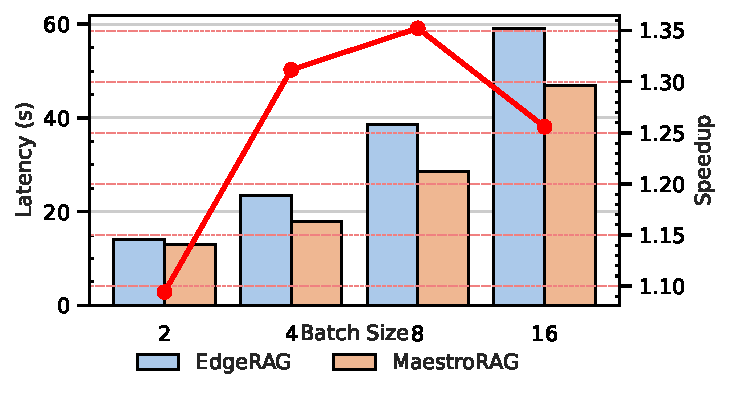
\includegraphics[width=0.9\linewidth]{Figs/JetsonThemVsUs.pdf}
  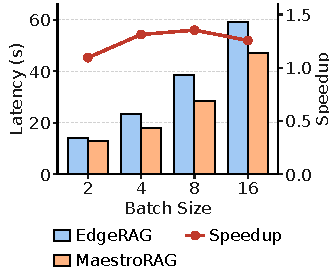
\includegraphics[width=\linewidth]{Figs/cr/JetsonThemVsUs.pdf}
  \caption{Latency comparison of EdgeRAG and \design{} on a Jetson~AGX~Orin with 1\,M database.}
  \label{fig:JetsonThemVsUs}
  \vspace{-10pt}
\end{wrapfigure}
we eliminate large data copies and cut overhead relative to EdgeRAG by 25\%--35\%. Although gains are smaller than on larger GPUs, they illustrate that our pipeline and data-sharing optimizations still yield meaningful benefits on edge devices.

\begin{figure*}[t]
    \centering
% CR-REPLACED: 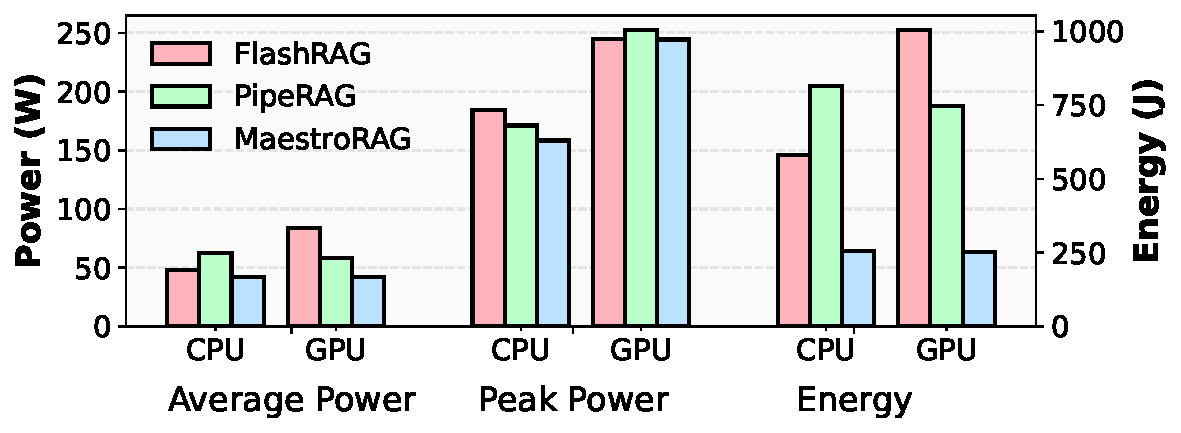
\includegraphics[width=0.8\linewidth]{Figs/power_energy_comparison.pdf}
    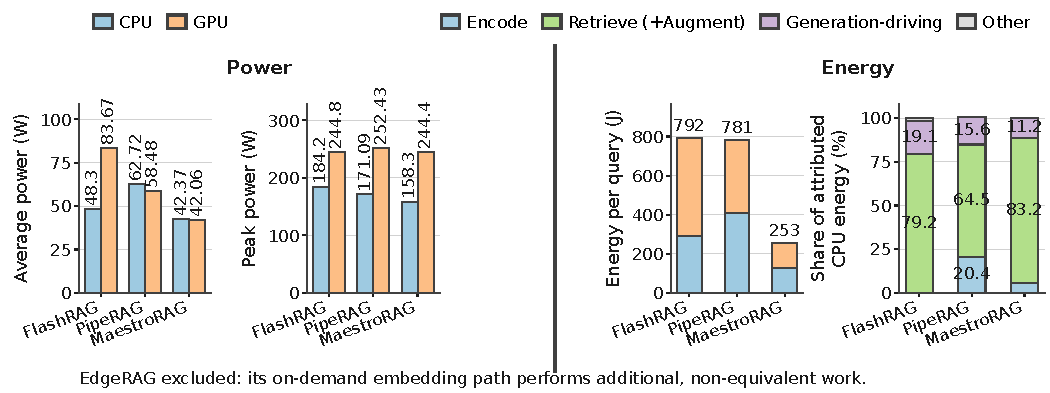
\includegraphics[width=\linewidth]{Figs/cr/fig6_power_energy_breakdown.pdf}
    \caption{\new{Power and energy on the Intel i9-14900K platform with an RTX\,4090 GPU at \texttt{BS=2}, \texttt{DB=4\,M}, and \texttt{top-k=5}. Left of the rule, average and peak power for the CPU and the GPU. Right of the rule, energy per query and the composition of CPU energy by pipeline stage. Power and energy are measured at the CPU package and at the GPU board. The composition is a share of idle-subtracted CPU package energy with DRAM excluded, so it is drawn on its own normalized axis rather than stacked onto the absolute joules beside it. \edgeRAG{} is excluded throughout.}}
    \label{fig:powerEnergyPlot}
    \vspace{-10pt}
\end{figure*}

% %%%%%%%%%%%%%%%%%%%%%% OLD LATENCY RESULT %%%%%%%%%%%%%%%%%%%%%%
% \subsection{Main Latency Results}
% \label{sec:main-latency-results}
% \Cref{Fig:MainLatencyResults2} reports end-to-end latencies for \design{} and three baselines on (i)~an RTX\,4090 with a 4\,M database at \texttt{BS=8}, (ii)~an RTX\,4080 also at \texttt{BS=8} and 4\,M, and (iii)~Jetson~AGX~Orin with 1\,M at \texttt{BS=8}. \textcolor{violet}{We also show a ``w/ Cache'' variant of our pipeline to illustrate multi-level caching benefits (\Cref{sec:Design:Caching})}. On the RTX\,4090, our method completes inference in 6.50\,s, which is 3--4$\times$ faster than \flashRAG{} (16.39\,s) or \pipeRAG{} (19.80\,s), and $\ge4\times$ faster than \edgeRAG{}. \textcolor{violet}{Enabling caching further cuts the latency to under 1\,s for repeated or similar queries, resulting in order-of-magnitude gains in typical round-trip time}. On the RTX\,4080, our pipeline finishes in 3.96\,s, outdoing \edgeRAG{}, \flashRAG{}, and \pipeRAG{} by up to 8.8$\times$, 1.9$\times$, and 5.4$\times$, respectively. On Jetson~AGX~Orin at \texttt{BS=8} and 1\,M, \design{} lowers latency to 28.56\,s, a 1.35$\times$ improvement over \edgeRAG{} (38.62\,s), even under a tight 15\,W power cap and limited CPU/GPU capacity. 
% %Although Jetson’s absolute latencies are higher, these findings confirm our pipeline’s robustness and memory-aware design across heterogeneous hardware.
% \textcolor{violet}{Finally, we compare our caching design to \edgeRAG{} \cite{EdgeRAG} under exact- and similarity-matching scenarios (\Cref{tab:cache_results}). The experimental configuration employs a fixed time to live (TTL) of 300 seconds and cache size of 32 prompts with 5 retrieval elements per prompt. Database sizes are as specified in the respective column headers, and batch size is held constant at 1 to maintain consistency with EdgeRAG's implementation parameters. For similarity matching, the results are averaged across multiple execution runs under conditions where 80\% of queries exhibit similarity scores exceeding the predefined threshold, thus generating partial cache hits. In exact matching, our pipeline and data management outperform EdgeRAG's
% %\edgeRAG{}'s 
% frequent embedding generations. However, in similarity matching ($\ge0.9~cosine$ similarity), the tail-end of requests faces higher retrieval latency, pushing average execution time towards a full flat index lookup, yielding inferior latency relative to \edgeRAG{}.}
% %which uses tree-based IVF indexing.
% %%%%%%%%%%%%%%%%%%%%%%%%%%%%%%%%%%%%%%%%%%%%%%%%%%%%%%%%%%%%%%%%%% 
\subsection{Main Latency Results}
\label{sec:main-latency-results}
\Cref{Fig:MainLatencyResults2} reports end-to-end latencies for \design{} and three baselines on 
(i)~an RTX\,4090 with a 4\,M database at \texttt{BS=8}, 
(ii)~an RTX\,4080 also at \texttt{BS=8} and 4\,M, and 
(iii)~Jetson~AGX~Orin with 1\,M at \texttt{BS=8}.
On the RTX\,4090, our method completes inference in 6.50\,s, which is 3--4$\times$ faster than \flashRAG{} (16.39\,s) or \pipeRAG{} (19.80\,s), and $\ge4\times$ faster than \edgeRAG{}\new{, whose stage-level composition is given in \Cref{sec:breakdown}}.
On the RTX\,4080, our pipeline finishes in 3.96\,s, outperforming \edgeRAG{}, \flashRAG{}, and \pipeRAG{} by up to 8.8$\times$, 1.9$\times$, and 5.4$\times$, respectively. 
On Jetson~AGX~Orin at \texttt{BS=8} and 1\,M, \design{} lowers latency to 28.56\,s, a 1.35$\times$ improvement over \edgeRAG{} (38.62\,s), even under a tight 15\,W power cap and limited CPU/GPU capacity. 
We also measure tail latency and amplification (\textit{P99}, \textit{P99/P50}) at \texttt{BS=8}, \texttt{DB=2\,M}. Our system achieves 5.26\,s (1.04), outperforming FlashRAG (14.86\,s, 1.14) and PipeRAG (14.41\,s, 1.09).
%At \texttt{BS=8}, \texttt{DB=2\,M}, our P99 latency/amplification is 5.26\,s (1.04), vs. 14.86\,s (1.14) for FlashRAG and 14.41\,s (1.09) for PipeRAG.
These findings confirm that our pipeline achieves robust, memory-aware performance across heterogeneous platforms.

\subsection{Throughput Evaluation}
\label{sec:throughput}
To assess throughput, we simulate bursty traffic from scaled Azure traces~\cite{azureTrace}, processing 256 queries on the RTX\,4090 and 128 in Jetson, injected every 10\,s and 15\,s, respectively. As shown in \Cref{Fig:ThroughputResults}, we set \texttt{DB=4\,M} and \texttt{BS=8}, consistent with the mid-scale latency experiments. On the RTX\,4090, \design{} reaches 1.60\,QPS, clearly ahead of \edgeRAG{} at 0.29\,QPS, \flashRAG{} at 0.68\,QPS, and \pipeRAG{} at 1.19\,QPS. Although the latter two are more GPU-conscious, they still incur frequent data movements and memory overheads that collectively restrict concurrency under large-batch bursts. In contrast, our CPU-based encoding and retrieval allow asynchronous, multi-query execution without overburdening GPU memory. In Jetson, \design{} achieves 0.43\,QPS, which is 6.7$\times$ better than \edgeRAG{} (0.064\,QPS) and about 1.16$\times$ faster than \pipeRAG{} (0.37\,QPS). \flashRAG{} relies on vLLM, which is not supported on Jetson; so, it is omitted. Despite the overall lower speed on the Jetson, our approach clearly shows that decoupling retrieval and encoding on the CPU increases concurrency under limited DRAM, thus sustaining higher steady-state throughput. These gains highlight the importance of a fine-grained pipeline with minimal CPU--GPU transfers, which helps the system respond more gracefully to bursty arrivals.
%instead of only single-query patterns.

\subsection{Power/energy efficiency}
To assess the real-world feasibility of \MR~\,in terms of energy consumption on edge platforms, we perform a complete power/energy profile of both the CPU and the GPU.
%, with results presented in \Cref{sec:additionalInsights}. 
For CPU 
%\red{(socket only, as it is difficult to measure exact DRAM power) }
power measurement, we employ \texttt{turbostat} utility~\cite{turbostat}, which provides hardware-based power consumption data by accessing Model-Specific Registers and Running Average Power Limit counters. This approach delivers package- and core-level power measurements with sampling at a 10Hz frequency.  GPU power consumption is measured using the \texttt{nvidia-smi}, which queries on-board power sensors to obtain instantaneous power draw at \emph{20Hz} sampling frequency. For the Jetson platform, we cap the power to $15W$ only, which is the lowest power setting offered on the particular platform representative of the handheld mobile devices used everyday.

The power and energy measurement results are plotted in \Cref{fig:powerEnergyPlot}. MaestroRAG significantly outperforms FlashRAG and PipeRAG in energy efficiency, only consuming $253.3J/query$, compared to \new{$792.00J$} and $780.92J/query$ for FlashRAG and PipeRAG, respectively. Moreover, FlashRAG and PipeRAG exhibit \new{$16.36\%$} and \new{$8.08\%$} higher peak CPU power usage, respectively.
\new{Attributing CPU package energy to pipeline stages, after subtracting idle package power and with DRAM excluded, gives $79.2\%$ retrieval and augmentation, $19.1\%$ generation-driving, and $1.8\%$ other for FlashRAG; $20.4\%$ encoding, $64.5\%$ retrieval, $0\%$ augmentation, and $15.6\%$ generation for PipeRAG; and $5.5\%$ encoding, $83.2\%$ fused retrieval and augmentation, and $11.2\%$ generation for MaestroRAG. These shares are of idle-subtracted energy, so they are reported as proportions rather than as a decomposition of the absolute totals above.}
%These findings confirm the efficiency advantages introduced by our design. 
The power consumption results for EdgeRAG are excluded from our evaluation due to implementation differences that preclude a fair comparison. EdgeRAG employs an on-demand embedding generation strategy that computes target cluster embeddings during cache misses, introducing additional computational overhead that substantially increases the system's power profile compared to MaestroRAG. \new{Because that path performs additional, non-equivalent work, a per-stage energy attribution for \edgeRAG{} would not be comparable with the other three systems.}
% While this design choice enables EdgeRAG to maintain a smaller memory footprint, it comes at the cost of increased latency and power consumption. Since EdgeRAG performs significantly more computation per inference run than our method, including these results would not constitute a fair comparison.}
%\cyan{
%Under iso-power settings,\ER incurs higher latency and performs more computations than \MR, 
%which clearly indicates greater average power consumption and overall energy usage.
%}

% \noindent\textbf{Summary of Latency and Speedup Findings.}
% Across all three platforms, our method improves total latency by factors ranging from $1.25\times$ to $12\times$ compared to prior RAG pipelines. While each system has its own resource idiosyncrasies, several high-level takeaways emerge:
% \textit{CPU--GPU co-design is key.} Offloading \emph{both} encoder and generator to the GPU, as in conventional designs, triggers large data transfers and heavy model loading overhead. We offload only generation, leaving embeddings and retrieval on the CPU.
% \textit{Memory-friendly partitioning prevents OoM.} Many baselines fail at \texttt{BS=16} and large databases, whereas our pipeline gracefully handles these cases, emphasizing the value of fine-grained partitioning.
% \textit{Moderate batch sizes yield best latency.} Oversized batches saturate memory bandwidth and cause I/O stalls, while too small batches underutilize compute resources. We found that \texttt{BS=4}--\texttt{8} is often optimal for end-to-end latency.
%  Although Jetson-class hardware is more limited, avoiding repeated GPU model loads remains beneficial, with up to a $1.35\times$ gain over EdgeRAG. 

% %%%%%%%%%%% DO WE NEED THIS?? %%%%%%%%%%%
% \subsection{Summary of Latency results:}%New
% \label{sec:overallLatencyPower}
% Our approach yields latency reductions of $1.25\times$--$12\times$ across three hardware platforms. Avoiding naive GPU offloading is crucial: we place only the generation stage on the GPU to limit data transfers and loading overheads, while CPU-driven retrieval and encoding prevent out-of-memory failures, even at \texttt{BS=16} with large databases. Further, moderate batch sizes (\texttt{BS=4}--\texttt{8}) strike the best performance balance, as oversized batches saturate I/O and small ones squander concurrency. 
% Although Jetson-class hardware is relatively constrained and possesses unified memory, where both the encoder and generation models are stored, applying the proposed software optimizations and distributing appropriate compute over CPU and GPU resources brings speedup of $1.35\times$ over EdgeRAG.
% %%%%%%%%%%%%%%%%%%%%%%%%%%%%%%%%%%%%%%%%%%%%%
% \begin{wrapfigure}{r}{0.65\linewidth}
%   \centering
%   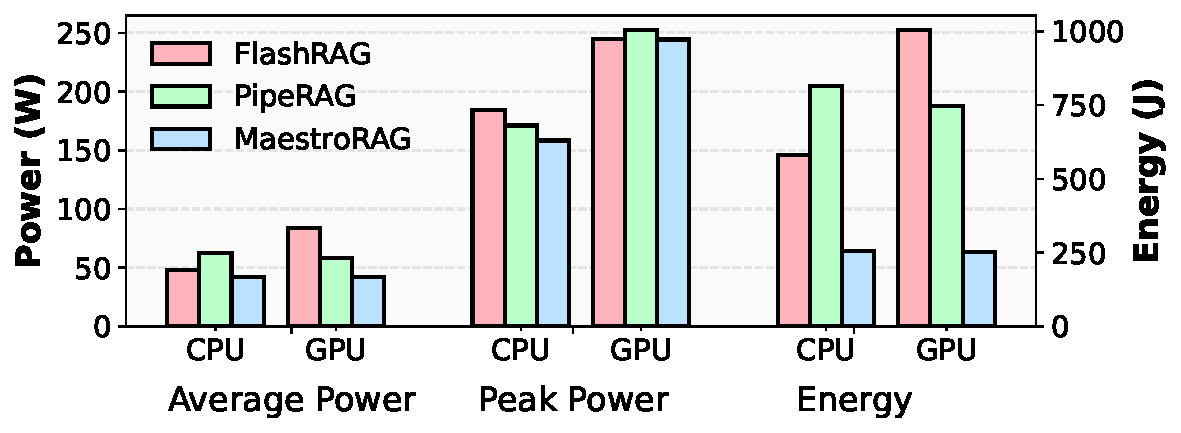
\includegraphics[width=0.95\linewidth]{Figs/power_energy_comparison.pdf}
%   \caption{Power and energy comparison of \design{} vs baselines.}
%   \label{fig:PowerEnergyWrap}
% \end{wrapfigure}


%%%%%%%%%%%%%%%%%%%%%%%%%%%%%%%%%%%%%%%%%%%%%%%%%%%%%%
 \begin{figure*} [ht!]
        \subfloat[Adaptive Worker Allocation]% in \design{}]
    {%
     % CR-REPLACED: 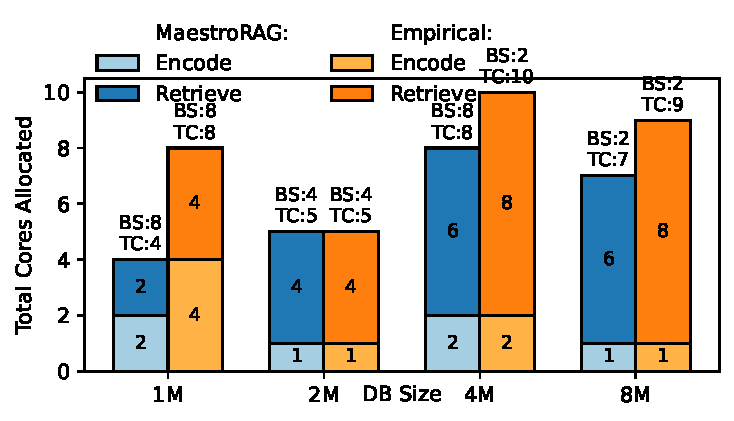
\includegraphics[clip,width=0.32\linewidth]{Figs/cores_allocation_stacked.pdf}%
     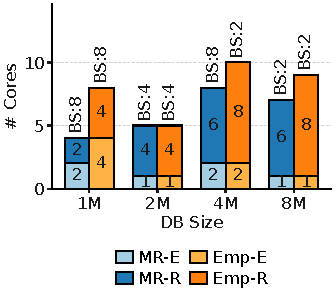
\includegraphics[clip,width=0.32\linewidth]{Figs/cr/cores_allocation_stacked.pdf}%
    \label{Fig:cores_allocation_stacked}
    }
    \hfill
    \subfloat[End to end latency comparison]% over all designs and devices]
    {%
    % CR-REPLACED: 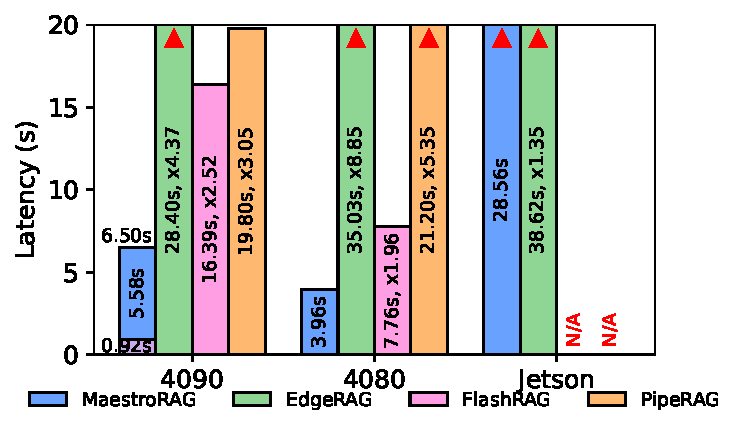
\includegraphics[clip,width=0.32\linewidth]{Figs/MainLatencyResults2.pdf}%
    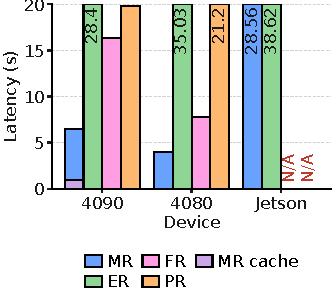
\includegraphics[clip,width=0.32\linewidth]{Figs/cr/MainLatencyResults2.pdf}%
    \label{Fig:MainLatencyResults2}
    }
    \hfill
    \subfloat[Throughput comparison]% over all designs and devices]
    {%
    % CR-REPLACED: 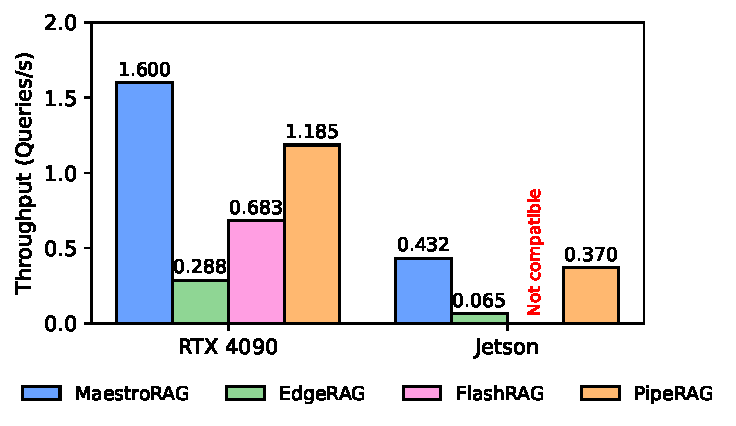
\includegraphics[clip,width=0.32\linewidth] {Figs/ThroughputResults.pdf}%
    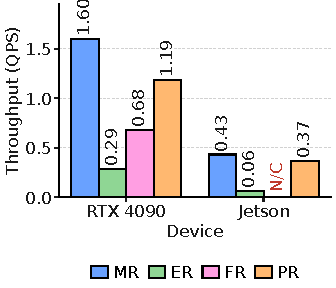
\includegraphics[clip,width=0.32\linewidth]{Figs/cr/ThroughputResults.pdf}%
    \label{Fig:ThroughputResults}
    }
    \caption{Key findings: (a) The adaptive worker allocation technique often results in better resource partitioning combinations to achieve the same latency/throughput. (b) End-to-end latency comparison for configurations selected by the adaptive worker allocator. (c) Throughput comparison for configurations selected by the adaptive worker allocator.}
    %\vspace{-0.1cm}
    \label{Fig:MainLatTputFigure}  
    \vspace{-10pt}
\end{figure*}
%%%%%%%%%% %%%%%%%%%% %%%%%%%%%% %%%%%%%%%%

% %%%%%%%%%%% DO WE NEED THIS?? %%%%%%%%%%%
% \subsection{Adaptive Batching and Worker Allocation}
% \label{sec:adaptive-mapper}
% In \Cref{Fig:cores_allocation_stacked}, we compare batch-size and core-allocation choices that our adaptive mapper (\Cref{subsec:resource-mapping}) recommends against the configurations uncovered by exhaustive grid searching. The bars labeled ``Mapper~Identified'' show the mapper’s suggested allocations, while the ``Empirically~Observed'' bars come from direct measurement. The results on the RTX\,4090 for four database sizes (1\,M, 2\,M, 4\,M, 8\,M) indicate that the mapper usually matches or outperforms purely empirical approaches, particularly at 2\,M and 4\,M. For instance, with a 4\,M database, the mapper selects \texttt{BS=8} and assigns 2~cores to encoding and 6~cores to retrieval, which indeed yields strong measured performance. Occasionally, as with 1\,M, the mapper opts for fewer encoding cores to keep the retrieval scaling robust. 
% %This suggests that e
% Exhaustive grid searches quickly become infeasible on real systems, especially as the database or query volume increases. In contrast, the mapper adapts well to new hardware or changing data sizes, making it especially useful in constrained environments that cannot afford extensive trial configurations.
% %%%%%%%%%% %%%%%%%%%% %%%%%%%%%% %%%%%%%%%%

%%%%%%%%%%%%%%%%%%%%%%%%%%%%%%%%%%%%%%%%%%%%%%%%%%%%%%
\begin{table}[]
%\vspace{-4pt}
\centering
\caption{Latency with caching. \design{}: MR; EdgeRAG: ER}
\resizebox{\linewidth}{!}{%
\begin{tabular}{lcccccc}
\toprule
& \multicolumn{2}{c}{2 mil} & \multicolumn{2}{c}{4 mil} & \multicolumn{2}{c}{8 mil} \\
\cmidrule(lr){2-3}\cmidrule(lr){4-5}\cmidrule(lr){6-7}
\textbf{Method} & \textbf{ER} & \textbf{MR} & \textbf{ER} & \textbf{MR} & \textbf{ER} & \textbf{MR} \\
\midrule
Exact & 2.033s  & 0.87s   & 2.0326s & 0.92s   & 2.0335s & 0.887s \\
Sim   & 2.047s  & 3.116s  & 2.003s  & 3.061s  & 2.138s  & 3.089s \\
\bottomrule
\end{tabular}%
}
%\caption{Latency with caching. \design{}: MR; EdgeRAG: ER}
\vspace{-10pt}
\label{tab:cache_results}
\end{table}

%%%%%%%%%%%%%%%%%%%%%%%%%%%%%%%%%%%%%%%%%%%%%%%%%%%%%%

% Finally, we compare the performance of our cache design against that of the EdgeRAG \cite{EdgeRAG} in two different scenarios: exact matching and similarity matching. While in exact matching, our superior pipeline and data-management dominates \edgeRAG{}'s frequent embedding generations, in similarity match, the tail-end of the request incur higher retrieval latencies This shifts our average execution time towards a complete lookup which is reflected as an inferior latency compared to \edgeRAG{}.
%We kept the threshold for similarity matching to be 0.9 which means that the incoming query should at least be 90\% similar to any of the previously cached queries. We observed that for exactly matching/recurrent queries, the latency is less than EdgeRAG. We attribute the execution time in this case to encoding of the query and cache lookup time. In case of partially matching (similar) queries, the execution time of our design is more compared to EdgeRAG 

\subsection{Software Caching}
\label{sec:software-caching}
To further reduce redundant computations and memory transfers, we exploit software caching in our design. By storing intermediate results in a cache, we avoid repeated operations such as costly vector similarity searches, thereby improving latency and throughput. Since edge deployments often process successive queries with overlapping context, caching naturally complements our design choices. This section outlines our caching strategies, adapted from previous work on cache-augmented generation~\cite{chan2024don}.

% \begin{figure}
% \centering
% 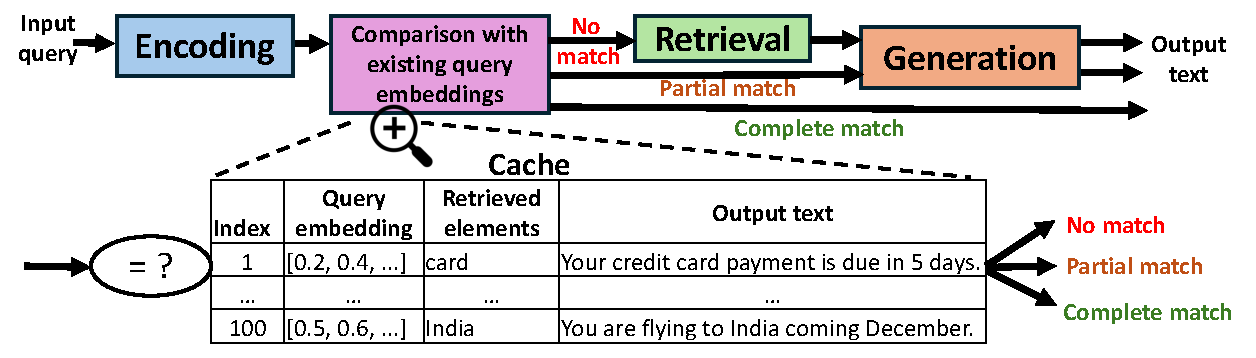
\includegraphics[width=0.7\columnwidth]{diagrams/caching_design.pdf}
% \caption{{Logical view of our caching scheme.}}
% \label{fig:caching_design} 
% \vspace{-20pt}
% \end{figure}

%A key component is 
\textit{Model caching}, where the encoding model is loaded once into a shared memory region, accessible to all workers, eliminates redundant memory copies and re-initialization overhead, accelerating query handling by avoiding frequent model load/unload cycles.
RAG workloads on edge might exhibit predictable patterns in query type, frequency, and likelihood (e.g. asking about the weather multiple times)
%, especially with small local knowledge bases
~\cite{EdgeRAG}. Although in practice this is highly application dependent, reusing previously fetched or generated data could significantly boost both performance and energy savings. We adopt two complementary data caching schemes.
%, shown in \Cref{fig:caching_design}.


\noindent\textbf{Similarity/Partial match retrieval caching:}  
For semantically similar queries, the system reuses prior retrieval results if the new query’s embedding exceeds a cosine similarity threshold (e.g., 90\%) with a cached embedding. Each cache entry stores the query embedding, retrieved documents, and a user-defined time-to-live (TTL). Thresholds and TTLs are tunable to balance factual accuracy and latency, as supported by~\cite{simThreshold, simThreshold2}. This scheme bypasses the retrieval phase, the most latency-intensive step, while still performing a fresh generation for nuanced differences.

\noindent\textbf{Exact/Complete match caching:}  
If a query matches a cached one exactly (embedding-based), the pipeline returns the stored final output directly, skipping both retrieval and generation. This assumes the vector database has not changed since the previous query, which is likely within the TTL window of a few minutes. This method is especially effective for repeated prompts, completely avoiding decoding overhead.

 \Cref{tab:cache_results} reports the results of our caching mechanisms under exact- and similarity-match scenarios. 
All experiments use TTL of 300\,s and cache capacity of 32 entries, each storing 5 retrieved documents per prompt. 
For a fair comparison with \edgeRAG{}, we adopt a batch size of 1.
%and maintain identical database sizes.
\new{Exact matching returns the cached final answer and skips both retrieval and generation, placing \design{} between 0.87\,s and 0.92\,s. Similarity matching reuses only the \topk{} retrieved documents and generates afresh for the new query, placing it between 3.06\,s and 3.12\,s. The difference between the two is therefore the cost of generation, which similarity matching still incurs; it is not a RAM-capacity effect. Against \edgeRAG{}, the residual gap in the similarity-match case is our process and thread handoff across workers, which adds approximately 1.1\,s. \edgeRAG{} does not incur this cost, since its execution is largely sequential and involves no process orchestration or thread synchronization. Because the measurement uses a batch size of 1, it compares our worst case against \edgeRAG{}'s nominal case; the handoff is a fixed per-batch cost, so we expect it to amortize at larger batch sizes.}
When 80\% of queries exhibit strong similarity, average latency improves substantially despite occasional cache misses.
On the Jetson~AGX~Orin (15\,W power cap), caching provides consistent speedups by avoiding redundant encoder invocations and memory transfers.
%, even under tight compute and memory budgets. 
%Compared to \edgeRAG{}, o
Our cache management exploits temporal and semantic locality. 
Overall, the cache policy provides a tunable, memory-efficient approach that leverages session-level query locality, yielding significant performance gains for interactive edge deployments.
\Cref{Fig:MainLatencyResults2} (purple stacked bar) showcases a pathological best-case exact match example on the RTX\,4090, where exact-match caching reduces latency from 6.50\,s to under 1\,s for repeated or highly similar queries.


%These caching strategies collectively minimize redundant computation, reduce power consumption, and improve responsiveness on edge platforms.

% %\label{sec:Design:Caching}
% Caching plays a vital role in reducing redundant computations and memory transfers in our RAG pipeline, especially on resource-limited devices. By selectively storing intermediate results in fast-access caches, we minimize repeated operations such as retrieval lookups, which consists of costly vector similarity searches, thereby improving both latency and throughput. Also, for our target deployment on edge devices, where the context of the successive queries largely remains the same, we believe caching is a natural progression in the set of design choices. This section outlines our caching strategies, drawing on key insights from prior work on cache-augmented generation~\cite{chan2024don} and adapting them for edge platforms with stricter memory and power constraints.

% \begin{figure}
% \centering
% 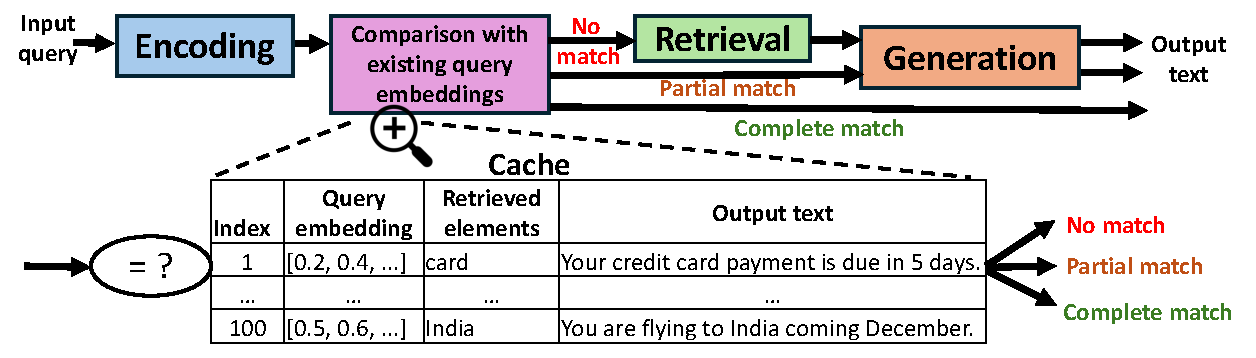
\includegraphics[width=1\columnwidth]{diagrams/caching_design.pdf}
% \caption{{Logical view of our caching scheme.}}
% \label{fig:caching_design} 
% \vspace{-10pt}
% \end{figure}

% A central feature of our design is \textit{model caching}, where we keep the encoding model resident in the main memory (or a shared memory region) across multiple parallel workers. Rather than loading the encoder separately for each worker, we store it once in a dedicated memory map. This approach eliminates redundant memory copies and shortens the model loading time, as the model weights need not be re-initialized on each query. 
% %Through this shared model cache, GPU (or CPU) resources are instantly accessible to multiple worker threads in turn, alleviating bottlenecks that arise from frequent load/unload cycles.

% The edge computation use cases are typically dependent on the user's interaction with the device, where patterns can be found about the nature, frequency, and the likelihood of the queries. Such patterns are even more vital in RAG use cases, where the database is local to an user and any set of queries are serviced only by the help of limited knowledge bases. The need to reuse the previously fetched/generated data becomes even more important as the likelihood of variation of the output given the same input is minimal with the added advantage of saving power. Thus, we propose two types of data caching schemes as depicted in \Cref{fig:caching_design}.

% \noindent\textbf{Similarity/Partial match based retrieval caching:} In this scheme, we recognize semantic similarity between queries and leverage the previously computed results to service the future queries provided the semantic similarity falls in an agreeable range. The system stores each query embedding along with its retrieved documents. When a new query arrives, its embedding is compared against cached embeddings using cosine similarity. If the similarity exceeds a configurable threshold (e.g., 90\%), the system reuses the previously retrieved documents, bypassing only the retrieval phase, while still performing the generation step. \red{This threshold, supported by recent research~\cite{simThreshold, simThreshold1, simThreshold2, simThreshold3}, is carefully chosen to preserve the factual accuracy of responses while improving latency. Retrieval relies on exact flat-indexing to maximize recall, ensuring that semantic similarity does not come at the cost of correctness. Each cache entry includes a user-configurable time-to-live (TTL), typically a few minutes, during which the entry is considered valid. Both the similarity threshold and TTL are tunable, allowing fine-grained control based on system requirements.} By using the prior similar query's retrieved elements, the RAG pipeline eliminates the most latency incurring operation, while still being able to cater to the newly arriving query's nuances through a fresh generation.  

% \noindent\textbf{Exact/Complete match caching:} The basis of this scheme is to detect the repeated queries coming to the pipeline over time. When a new query arrives, the encoding model generates embedding and does a cache lookup to find out the most similar previously serviced query. In case of exact match, the subsequent stages in the pipeline are bypassed, and the final generated output is given to the user. The primary assumption is that the state of the vector database since the service of the prior query to the arrival of this new query has not changed. Given that we we keep track of the \textit{time to live} of each of these cache entries, which is typically a few minutes, it is highly likely that the vector database remains the same. This caching avoids any repeated decoding overhead and is valuable when certain prompts are repeated verbatim during a user session.

%\vspace{-10pt}
\subsection{Additional Insights}
\label{sec:additionalInsights}
%Our evaluation is comprehensive and designed to demonstrate the robustness of our system under worst-case conditions. Beyond this baseline, 
Here, we provide additional results that highlight the adaptability and generalization capacity of our design across a range of sensitivity settings. These include experiments with more relaxed indexing strategies and more stringent configurations involving longer input context lengths.

\noindent\textbf{Latency results insights: }\design{} yields latency reductions of $1.25\times$--$12\times$ across three hardware platforms. Avoiding naive GPU offloading is crucial: we place only the generation stage on the GPU to limit data transfers and loading overheads, while CPU-driven retrieval and encoding prevent out-of-memory failures, even at \texttt{BS=16} with large databases. Furthermore, moderate batch sizes (\texttt{BS=4}--\texttt{8}) strike the best performance balance, as oversized batches saturate I/O and small ones squander concurrency. 
Although Jetson-class hardware is relatively constrained and possesses unified memory, where both encoder and generation models are stored, applying the proposed software optimizations and distributing appropriate compute over CPU and GPU resources brings a speedup of $1.35\times$ over EdgeRAG.

\noindent\textbf{Adaptive Batching and Worker Allocation: }In \Cref{Fig:cores_allocation_stacked}, we compare the recommended batch-size and core-allocation between our adaptive mapper (\S\ref{subsec:resource-mapping}) and exhaustive grid searching. The bars labeled ``Mapper~Identified'' show the mapper’s suggested allocations, while the ``Empirically~Observed'' bars come from direct measurement. The results on the RTX\,4090 for four database sizes (1\,M, 2\,M, 4\,M, 8\,M) indicate that the mapper usually matches or outperforms purely empirical approaches, particularly at 2\,M and 4\,M. For instance, with a 4\,M database, the mapper selects \texttt{BS=8} and assigns 2~cores to encoding and 6~cores to retrieval, which indeed yields strong measured performance. Occasionally the mapper opts for fewer encoding cores to keep the retrieval scaling robust. Exhaustive grid searches quickly become infeasible on real systems, especially as the database or query volume increases. In contrast, the mapper adapts well to new hardware or changing data sizes, making it especially useful in constrained environments that cannot afford extensive trial configurations.

\noindent\textbf{Impact of number of tokens: }To assess the scalability of our approach with respect to input length, we vary the number of input tokens while keeping all other hyper-parameters fixed. The encoding latency increases only $0.6\%$ when moving from 10 to 20 tokens, and $1.2\%$ at 100 tokens. Generation latency remains unchanged at 20 tokens and increases by $12\%$ at 100 tokens. Even with 100 tokens, the total input to the generation module (query and the top-5 retrieved passages) exceeds 500 tokens, indicating the system’s resilience to context length expansion.

\noindent\textbf{Impact of indexing schemes: }In addition to the flat indexing scheme for accessing the database, we also experimented with three other indexing schemes---approximate nearest neighbor (ANN) methods~\cite{faiss}, IVF-Flat, IVF-PQ, and HNSW---to understand the performance implications. All alternatives provided substantial latency improvements, with observed gains of $29.27\%$, $28.15\%$, and $32.18\%$ respectively. This demonstrates the ability of our system to trade off between retrieval accuracy and latency via configurable indexing.

\noindent\textbf{Impact of optimization mechanisms: }To isolate the impact of individual optimizations, we performed an ablation study of end-to-end latency. Starting from a baseline latency of $15.12s$ (no optimizations), we observe incremental improvements: adaptive batching and core allocation reduce the latency to $11.79s$; software-level optimizations bring it down further to $6.497s$; and (effective) caching achieves $2.003s$. These results clearly demonstrate the effectiveness of our layered optimizations.

\new{\noindent\textbf{Portability of optimizations to baselines: }We ported the transferable optimizations to \pipeRAG{}: memory-mapped indices, warm encoder weights in DRAM, and persistent thread and core pinning. For an isolated batch at \texttt{BS=1}, the optimized \pipeRAG{} reaches 0.22\,s for encoding, 1.55\,s for retrieval, and 0.10\,s for augmentation, close to \design{}. Under the steady-state bursty Azure trace of \Cref{sec:throughput}, it reaches 1.38\,QPS against our 1.60\,QPS, still runs out of memory at \texttt{BS=16}, and suffers head-of-line blocking because its synchronous stages cannot admit the next batch independently. The remaining benefit comes from asynchronous multi-width orchestration, worker scaling, and adaptive batching.}

\noindent\textbf{Impact of cold start: } Finally, we evaluate cold-start overhead which consists of latency incurred in model loading, process creation by scheduler for different stages, index loading and other library loads. MaestroRAG incurs a one-time cold-start cost of $7s$ comprising $0.36s$ for encoder loading, $3.04s$ for vector index construction, and $3.36s$ for loading the generation model onto the GPU. In contrast, FlashRAG and EdgeRAG re-incurs this overhead at the beginning of every batch, highlighting a key advantage of our initialization strategy in batch inference settings.


% \subsection{Additional Results}
% Our evaluation is exhaustive, demonstrating the performance of our system even under worst-case scenarios. In addition to this, we present supplementary results to highlight the flexibility and capability of our design across varying degrees of sensitivity. This includes the use of alternative, more lenient indexing strategies as well as stricter configurations with extended context lengths. Furthermore, we provide a detailed analysis of power consumption, showcasing how different components and design choices contribute to overall efficiency improvements. This analysis also includes an ablation study to isolate and quantify the impact of each approach.


% With all other hyper-parameters frozen, encoding latency rises just 0.6\% from 10 to 20 tokens and only 1.2\% at 100 tokens; generation is unchanged at 20 tokens and increases 12\% at 100 tokens. (The total input to generation stage is top-5 passages + input query. So system is still getting 500+ tokens.)

% We used flat-indexing for accuracy and benchmarked three popular alternatives—IVF-Flat, IVF-PQ, and HNSW—observing performance gains of 29.27\%, 28.15\%, and 32.18\%, respectively, wrt flat-indexing. 

% We conducted power measurements and found MaestroRAG to be more efficient than FlashRAG in terms of average power, peak power and total energy consumed.MaestroRAG consumes 253.3J/query vs 791.8J(+212.6\%) of FlashRAG. We also observed FlashRAG has 16.45\% more peak CPU-power.

% We observe: Communication latency: 3.36s; No optimization:15.12s, +Adaptive-batching and core allocation:11.79s, +Software optimizations: 6.497s, +Caching: 2.003s. Cold-start costs(Rev-B): MaestroRAG’s cold-start is 7s: 0.36s for encoder-load, 3.04s to build vector-indices, and 3.36s to move the generation-model to the GPU. This overhead is one-time before the first batch; FlashRAG re-incurs cold-start with every batch.
% \subsection{Adaptive Batching and Worker Allocation}
% \label{sec:adaptive-mapper}

% We begin by illustrating how our adaptive mapper (Section:~\S\ref{subsec:resource-mapping}) identifies favorable (\textit{batch-size}, \textit{core-allocation}) configurations versus what we observe with empirical grid searches. 
% \Cref{Fig:cores_allocation_stacked} showcases representative results for four database sizes---1\,M, 2\,M, 4\,M, and 8\,M---on the RTX\,4090 platform.
% % \paragraph{Mapper vs.\ Empirical Observations.} 
% In \Cref{Fig:cores_allocation_stacked}, the bars labeled 
% ``Mapper~Identified'' are the allocations suggested by our model-based approach, while the ``Empirically~Observed'' entries are derived from a more exhaustive measurement search. Across most configurations (e.g. 2\,M and 4\,M), the mapper's recommendations agree with or improve upon the empirically measured settings. For example, at a 4\,M database, the mapper selects \texttt{BS=8}, $2$~cores for encoding, and $6$~cores for 
% retrieval---which we find also yields strong measured results. 
% In certain cases (e.g. 1\,M), the mapper picks a slightly smaller encode-core count, reflecting that it is preferable to keep retrieval parallelism balanced with encode concurrency.
% We emphasize that \emph{purely empirical} searches become impractical on real systems for large parameter spaces, especially as the database or number of queries grow. By contrast, our model-based mapper adapts quickly to new hardware or changes in data size. This adaptability is particularly beneficial in resource-constrained environments, where launching many trial configurations to find an optimal setting would be costly or infeasible.

% \subsection{Main Latency Results}
% \label{sec:main-latency-results}
% \Cref{Fig:MainLatencyResults2} summarizes the end-to-end RAG latency for our design and the baselines on three platforms: 
% (i)~RTX\,4090 with a 4\,M database at \texttt{BS=8}, ii)~RTX\,4080 with a 4\,M database (also \texttt{BS=8}), and (iii)~Jetson~AGX~Orin with a 1\,M database at \texttt{BS=8}. For our pipeline, we also evaluate a variant (\emph{Ours w/ Cache}), highlighting the gains from our multi-level caching scheme (Section~\S\ref{sec:Design:Caching}). On the \textbf{RTX\,4090}, our method completes inference in $6.50\,\mathrm{s}$, nearly $3\times$--$4\times$ faster than \flashRAG{} ($16.39\,\mathrm{s}$) or \pipeRAG{} ($19.80\,\mathrm{s}$), and over $4\times$ faster than \edgeRAG{} ($28.40\,\mathrm{s}$). Enabling caching drives the latency down to under $1\,\mathrm{s}$ for many repeated or similar queries, effectively cutting typical round-trip times by an order of magnitude.
% On the \textbf{RTX\,4080}, we see a similar pattern: our pipeline reaches $3.96\,\mathrm{s}$, outperforming \edgeRAG{}, \flashRAG{}, and \pipeRAG{} by up to $8.8\times, 1.9\times$, and $5.4\times$ respectively. Finally, on the \textbf{Jetson} device with \texttt{BS=8} and a $1\,\mathrm{M}$ database, our design runs in $28.56\,\mathrm{s}$, beating \edgeRAG{}'s $38.62\,\mathrm{s}$ by roughly $1.35\times$. Although the absolute latencies are larger on Jetson, the gain is still notable under tight power (15\,W) and limited CPU/GPU resources. 
% Together, these findings confirm that our pipeline remains robust and memory-friendly across diverse hardware.

% \subsection{Throughput Evaluation}
% \label{sec:throughput}
% We next evaluate \emph{throughput}, measured in queries served per second, under a bursty workload derived from scaled Azure traces. Specifically, we process $256$~queries on the RTX\,4090 and $128$~queries on Jetson, injected at intervals of $10\,\mathrm{s}$ and $15\,\mathrm{s}$,respectively. As shown in \Cref{Fig:ThroughputResults}, we fix \texttt{DB=4\,M} and \texttt{BS=8} to match the mid-scale latency tests on desktop GPUs.

% On the \textbf{RTX\,4090}, our pipeline achieves a throughput of $1.60$~QPS, compared to $0.29$~QPS, $0.68$~QPS, and $1.19$~QPS for \edgeRAG{}, \flashRAG{}, and \pipeRAG{}, respectively. Although the latter two baselines are more GPU-conscious than \edgeRAG{}, they still incur significant data transfers and memory overhead, limiting concurrency when large batches arrive in rapid bursts. Our pipeline, by contrast, executes encoding and retrieval in separate CPU workers, enabling multiple queries to be processed asynchronously without oversubscribing GPU memory.

% On the \textbf{Jetson}, we obtain $0.43$~QPS, a $6.7\times$ improvement over \edgeRAG{} ($0.064\,\text{QPS}$) and $1.16\times$ that of \pipeRAG{} ($0.37\,\text{QPS}$).
% \flashRAG{} relies on vLLM for model execution, which is currently incompatible with Jetson’s hardware stack; hence no results are reported there. Despite the slower device speed overall, it is clear that \emph{modular} CPU-based retrieval and encoding help sustain higher in-flight queries under limited DRAM, raising steady-state throughput.

% \noindent\textbf{Key Takeaways.} These throughput results confirm that our approach’s fine-grained pipeline---with CPU-based embedding and retrieval plus minimal GPU transfers---not only reduces latency for single-query batches but also scales more gracefully to bursts of concurrent queries. This is critical in real-world  edge scenarios, where traffic often arrives in bursts rather than in evenly spaced singletons. 
%By avoiding repeated model loading and GPU memory oversubscription, our pipeline maintains high query throughput and meets SLO requirements for both desktop-class and embedded devices.
%%%%%%%%%%%%%%%%%%%%%%%%%%%%%%%%%%%%%%%%%%%%%%%%%%%%%%
% Text matter end


%%%%%%%%%%%%%%%%%%%%%%%%%%%%%%%%%%%%%%%%%%%%%%%%%%%%%%
%  \begin{figure} 
%     \subfloat[End to end latency of \design{} on RTX 4080]
%     {%
%      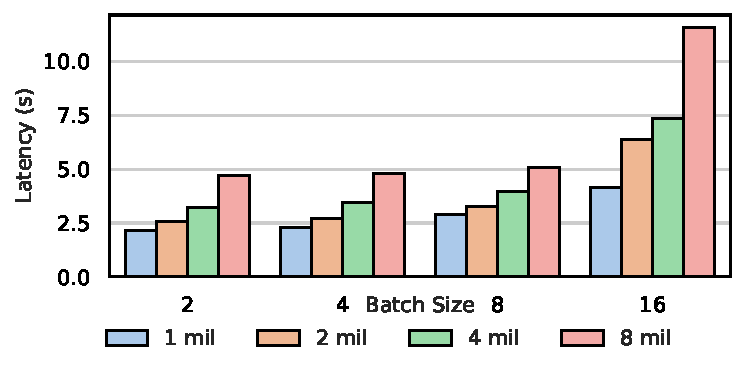
\includegraphics[clip,width=0.8\linewidth]{Figs/4080Latency_Ours.pdf}%
%     \label{Fig:4080Latency_Ours}
%     }
    
%     \subfloat[Speedup observed by \design{} over baselines.]
%     {%
%     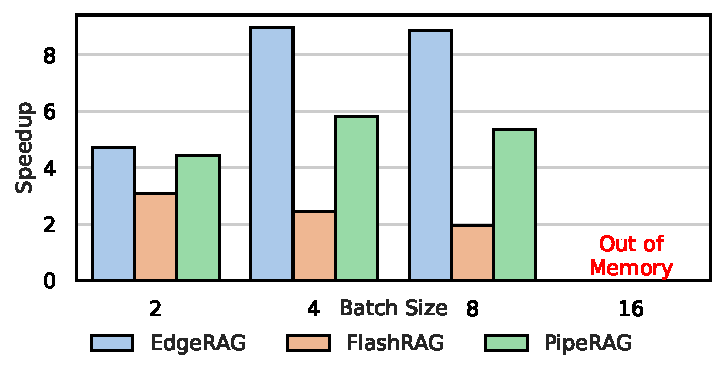
\includegraphics[clip,width=0.8\linewidth]{Figs/4080Speedup_Merged.pdf}%
%     \label{Fig:4080Speedup_Merged}
%     }
%     \caption{Latency study on RTX 4080: (a) Latency of our design on an RTX 4080 for various batch sizes and database sizes. Latency grows moderately as batch size and dataset scale increase, culminating in the highest times at 16-batch and 8\,million entries. (b) Speedup of \design{} over EdgeRAG, FlashRAG, and PipeRAG at 4\,million entries on an RTX 4080. For batch sizes up to 8, \design{} yields up to an 8.97$\times$ improvement (EdgeRAG), while the other frameworks run out of memory at batch size 16, highlighting our method's superior scalability.}

%     %\vspace{-0.1cm}
%     \label{Fig:Latency4080}  
%     %\vspace{-0.5cm}
% \end{figure}
%%%%%%%%%% %%%%%%%%%% %%%%%%%%%% %%%%%%%%%%

%\section{Methodology}
%\label{sec:methodology}
%In this section, we give the details about the choice of our hardware, datasets, evaluation metrics and the baselines compared against. 

%\fixme{for different stages different batch sizes shine, and hence we use dynamic batching}

%~\textbf{Hardware Setup}: We perform experiments on the following three different hardware setups representative of the different consumer and edge grade devices: (i) Intel i9-14900K having 32 virtual cores (8 P-cores and 16 E-cores constituting the 24 physical cores) with 128 GB main memory, equipped with RTX 4090 GPU with 24 GB memory; (ii) Intel i9-14900F having aforementioned CPU core configuration and connected to an RTX 4070 GPU with 16 GB memory; and (iii) Nvidia Jetson AGX Orin developer kit with 64 GB main memory~\cite{nvidia_jetson_orin}. We believe  these devices are representative of the personal computing devices available to the users today. 

%~\textbf{Datasets and Models}: We use Wikipedia corpus dump~\cite{wikipedia_corpus_dump} for knowledge retrieval database and it is indexed using FAISS library~\cite{faiss} to create a flat indexing scheme where "L2 distance" is used as a similarity metric for top k item selection with respect to the input prompt. The input prompts used for query are from Google's Natural Question Dataset~\cite{natural_questions}. Since there is no publicly available trace representative of RAG use-pattern on personal computing devices, we use bursty traces from Azure scaled down to fit smaller computational footprint matching the consumer-grade device capabilities. The text-to-embedding generation model used to generate the embeddings for the database and the incoming queries is e5-base-v2\cite{e5_base_v2}. The models used for inference are Llama-3.1-8B-Instruct\cite{llama_3_1_8b_instruct} and OPT 2.7B\cite{opt} on the RTX 4090 and RTX 4070 GPUs, respectively. We choose a smaller model Llama-3.2 1B\cite{llama3_2_1b} model to run on Jetson AGX Orin development board.

%~\textbf{Metrics}: 
%Since the target application is mostly user facing on a resource constrained personal computational platform, 
%We use (i) latency, (ii) hardware utilization, and (iii) throughput as the primary metrics in out evaluations. 

%~\textbf{Baselines}: The baselines chosen to compare the proposed design against are (i) FlashRAG\cite{jin2024flashrag} which presents an end-to-end RAG pipeline and evaluation framework where the encoding and generation stages take place on GPU, and (ii)  PipeRAG\cite{jiang2024piperag} that introduces pipelining at server-scale computing. Note that none of these prior approaches  addresses the underlying resource underutilization issue,  which becomes even more critical in personal computational devices like laptops, tablets, and smartphones. 

%%%%%

% \subsection{Evaluation Results and Insights}
% Using real-system measurements, we evaluate the benefit of our \design{} for achieving optimal resource allocation (Section~\ref{sec:optimization_design}).  As shown in Figure~\ref{}, we observe the trend of overall execution time for different batch sizes of requests across varied database sizes. As the overall work (in terms of batch sizes and database size to lookup) grows, the execution time reflects the corresponding trend of growth of latency that comprises of compute and IO times. The comparisons of the execution times of \design{} with the state-of-the-art RAG pipelines have been depicted in the Figurexxxxxxx where we observe that the speedup of our design over EdgeRAG increases from batch size of 2 to 8 across all database sizes. The speedup drops at batch size of 16 as the end to end latency of our design increases rapidly owing to the huge IO costs that 16 requests put on the main memory. It is worth noting that \design{} reports latency over retrieval through flat indices whereas the EdgeRAG scheme works with IVF indices which are coarser in nature compared to the exhaustive flat indices. Multiple vectors are clustered together to form one centroid in IVF which reduces the search complesity in case of retrieval very significantly. Even then \design{} fairs better compared to EdgeRAG across all batch size and database settings.
% Figure~\ref{xxxxxxxx} shows the speedup of \design{} over FlashRAG that uses GPU for encoding as well as generation stage. The speedup in this case shows an interesting trend. The speedup for 1 mil database size increases with increase in batch size whereas the speedup for 8 mil database size drops as batch sizes grow. This is primarily due to the domainance of retrieval time in end to end latency for bigger database sizes that entails more vector similarity computation over limited CPU cores. But in case of smaller database sizes like 1 mil, the 


%\subsection{Key Results on RTX 4090}
%\subsubsection{Benefits on RTX 4090}
%Fig.~\ref{fig:4090_latency_improvement_piperag} shows the latency improvement brought by our proposed design over PipeRAG~\cite{jiang2024piperag} under various batch and database sizes. We note that latency improves by up to 1.77x (batch size of 2 and database size of 1 million), leading to an average performance uplift of 1.44x. Similarly, as plotted in  Fig.~\ref{fig:4090_latency_improvement_flashrag}, when compared against FlashRAG~\cite{jin2024flashrag}, our proposed design produces latency improvements. Particularly, it achieves a maximum gain of 1.69x, and an average gain of 1.16x. In general, the speedup is higher with smaller database sizes, and large batch sizes. Our observations reveal that as the database size grows, the retrieval stage time increases as a result of increased number of indices to exhaustively compare with. This also increases the corresponding IO operations that the retrieval stage entails and hence pipeline becomes imbalanced again. 

%Fig.~\ref{fig:4090_throughput} compares the throughput of our proposed design with PipeRAG and FlashRAG. We see that our approach  achieves a 1.2x and 3x improvements over PipeRAG and FlashRAG, respectively. The throughput is measured with database size of 1M size and batch size of 8. Finally, Fig.~\ref{fig:4090_utilization} evaluates the utilization for various batch sizes. Our proposed scheme achieves an average utilization of 86\%. On average, our design achieves a 24\% higher throughput than PipeRAG, and 74\% higher utilization than FlashRAG. 

%\subsection{Key Results on RTX 4070}
%We next evaluate various schemes on another consumer-grade GPU:  RTX 4070. Fig.~\ref{fig:4070_results} highlights the latency and throughput benefits. Since this GPU has a smaller main memory capacity (16 GB) compared to RTX 4090, a model like Llama 8B overshoots this when loaded along with necessary input data. To resolve this issue, we change the model of choice to OPT 2.7B which allows the model, input data as well as intermediate KV cache to reside without overshooting this limit. Even with the said modification, we note that PipeRAG and FlashRAG fail to run with a batch size of 16, owing to static batching of prompt. However, our proposed design runs on this GPU with the large batch size of 16 as the generation scheduler handles such possible issues by only launching batches that fit within the GPU main memory capacity. On an average, we note a latency improvement of 1.38x with respect to the two prior works (PipeRAG and FlashRAG). Further, in terms of throughput, we note that our proposed design outperforms FlashRAG and PipeRAG by 3.22x and 1.09x,  respectively. 

%\subsection{Key Results on Jetson Orin}
%Given that the deployment of RAGs on edge devices like mobile phones has gained momentum in recent times, we also evaluate our proposed design on Jetson AGX Orin platform. We could not compare it with FlashRAG since the setup requires cerrtain libraries, which are not compatible for ARM ISA. Thus, we only report our comparison with PipeRAG. Fig.~\ref{fig:jetson_result} highlights the latency improvements brought by our proposed design. It can be seen that, at a batch size of 16, the PipeRAG design fails to run due to current throttling issue. Overall, our design achieves a maximum gain of 1.65x and an average gain of 1.24x. 
